\documentclass[10pt,a4paper,notitlepage]{report}
\usepackage[utf8]{inputenc}
\usepackage{amsmath}
\usepackage{amsfonts}
\usepackage{amssymb}
\usepackage{hyperref}
\usepackage[margin=1in]{geometry}
\usepackage{fancyhdr}
\usepackage[svgnames]{xcolor}
\usepackage{graphicx}

\pagestyle{fancy}
\fancyhead[L]{\small Decoding Neuronal EEG Activity}
\fancyhead[R]{\small\textsc{Problem 1}}
\renewcommand{\headrulewidth}{0.4pt}
\fancyfoot[C]{\thepage}

%\newcommand{\code}[1]{\colorbox{lightgray}{\texttt{#1}}}

\begin{document}

??? GENERAL NOTES ON SUBMISSION, GRADING, ETC. ???

The programming problems consist in filling the gaps in the provided scripts according to the problem description and the comments within the code. The missing parts are typically indicated by '\texttt{...}' (not to be confused with line breaks!), whereas each '\texttt{...}' might be replaced by multiple lines of code. Following the provided code is recommended but only leads you to one of many possible solutions. If some part of the code seems unclear or counterintuitive to you, feel free to depart from it. Be aware, however, that the suggested variable names and structures are typically used later in the script, e. g. for plotting, and occur again in other scripts and problems. In any case, your code should produce the same output as the Musterlösung. \textbf{Note}: To be able to run the code, you must have the folder \texttt{utility} and all subfolders as well as the location of the ECG/EEG datasets added to your MATLAB path.

\section*{Main Script}
In this problem, you will generate bivariate random data from two normal distributions and classify the data accordingly using logistic regression. The script \texttt{runTest.py} provides the main parameters.

\begin{enumerate}

\item First, you have to produce the data using these parameters and an appropriate function, concatenate the two sample populations, and create a vector of labels (ones for one population, zeros for the other). \texttt{X} will be a 2*\texttt{nSamples}$\times$2 matrix and \texttt{L} will be of length 2*\texttt{nSamples}.

\item Next, we want to see what the two underlying distributions look like along the two data dimensions $x_1$ and $x_2$ (not to be confused with the two sample populations \texttt{X1} and \texttt{X2}). Create a grid of 100$\times$100 equidistant points within the bounds of the sample populations, using \texttt{xVector}, and compute the two PDFs for each point. (If you have trouble with the suggested one-liners, use for-loops instead.) The result \texttt{pDist} should be a 100$\times$100 matrix containing the sum of both PDFs.

\item Now we train a General Linear Model (GLM) on the sample data. For this we need to install an extra package:
\begin{itemize}
  \item \textbf{statsmodels} has a GLM implementation for different link functions.
  \item \textbf{sklearn} has a logistic regression implementation.
  \item \textbf{pyglmnet} is a special puropose package for all kinds of GLMs.
\end{itemize}


\item To display the decision boundary of the fitted model, we solve the iso-error problem, i. e. we compute the line on which $P(C_1|x) = P(C_2|x) = 0.5$. This means solving the equation
\begin{equation*}
0.5 = \sigma (w^Tx+w_0)
\end{equation*}
with $\sigma$ being the logistic function, $w=(w_1,w_2)$ together with $w_0$ given by the coefficients \texttt{coeff} we just computed, and $x=(x_1,x_2)$. We have to rewrite the equation for $x_2$ and set $x_1$ to \texttt{xVector}.

\item Now we validate the fitted model (find the appropriate function!) on the same 100$\times$100 data points as before to get the posterior densities predicted by the model. (We only compute $P(C_1|x)$, since $P(C_2|x)=1-P(C_1|x)$.)

\item Finally, we want to cross-validate the model, using our own function.

\end{enumerate}


\section*{Classification Function}
The file \texttt{modelFitVal.py} contains a function \texttt{modelFitVal}, which should take a data matrix, a correpsonding label vector, and the number of partitions, then iteratively divide the data and labels into training sets and test sets, fit and validate the GLM, and return the mean percentage of correctly predicted labels.

\begin{enumerate}
  \item Set up a vector of randomized partition tags with values 1 to \texttt{kPart} (e.g. \texttt{partTag = [2 1 4 3 1 3 ...]} for \texttt{kPart = 4}) and the same length as \texttt{X}.

  \item In the subsequent loop we divide the data and labels into test and training sets using this vector. In each iteration, select the test set via the current partition tag and the training set via the remaining \texttt{kPart-1} tags.

  \item Now you perform logistic regression as before and compare the rounded validation data, i. e. the predicted labels for the test data, to the actual labels. The percentage of correct predictions is then accumulated over iterations.
\end{enumerate}

\section*{Plotting and Exploring}
Your code should print the model's average classification performance and produce the two figures below, showing the sample data with their underlying distributions and the model's decision boundary, and the class posterior probabilities, respectively.

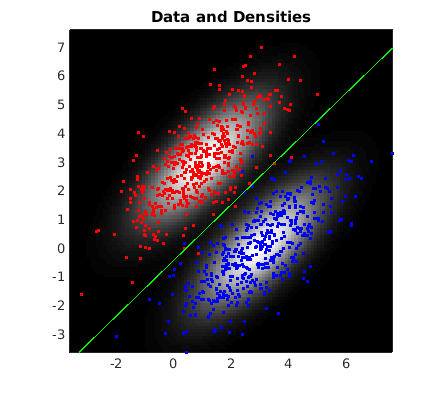
\includegraphics[scale=0.6]{p1fig1.png}
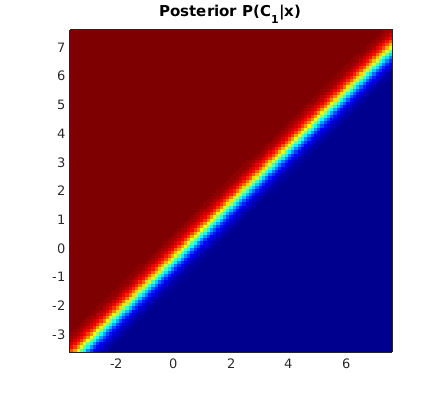
\includegraphics[scale=0.6]{p1fig2.png}

Note that the plots will vary a bit at between runs because of the randomness in sampling and cross-validation. Classification performance should be at or near 100 \%.

You may want to try different distribution parameters and sample sizes and see how performance and plots change. Try to understand the warning messages you might get.

\end{document}
